
\chapter{Manufacturing System Identification}
\label{cha:ident}
In this chapter, the identification process of the controlled system is
explained. This identification process can be divided in two parts: the data acquisition, where the inputs\slash outputs of the system are
  acquired, and the model identification, where the acquired data is
  used in the identification algorithm, \Autoref{alg:identification}, and the
  identified model is generated.
 
In the next sections these two parts are described.

\section{Data Acquisition}
There are multiple ways to obtain the values of the
inputs\slash outputs of a system. The data acquisition methods can be divided in two categories. In the first one,
the data is continuously registered, and in the second one the data is buffered
and registered in batches from time to time.
The first one is usually used for online processes, where the continuous flow of
information is necessary, and processes that are repeated
extensively. Examples of these processes are control loops and fault
detection modules. On the other hand, the second one is usually used for offline
processes, processes that are computationally expensive and sporadic processes.
An example of such processes can be modelling a big system, what can be a
resource-intensive task.

Since \Autoref{alg:identification} takes as input a set of paths, all the data is
acquired beforehand. The data can
be acquired in batches, and once all the data is collected, the algorithm can be
executed.

The most straightforward way to obtain the data from a Siemens \PLC{} is by
using data logs. The Siemens \PLC{} S7-1500 includes function blocks to
use inside a \LD{} to store custom data in a \CSV{} formatted file. This file is
saved in a SD card. In order to download this file to a computer, the SD card can be connected to a PC,
or the file can be downloaded using a web browser, if a Web Server is configured in the
\PLC.

The five function blocks used to log data are called
\verb|DataLogCreate|,
\verb|DataLogOpen|, \verb|DataLogWrite|, \verb|DataLogClose| and \verb|DataLogDelete|.
These blocks are shown in the \LD{} of \Autoref{fig:datalogcreate,fig:datalogopen,fig:datalogwrite,fig:datalogclose,fig:datalogdelete}.


% \begin{figure}[H] \centering
%  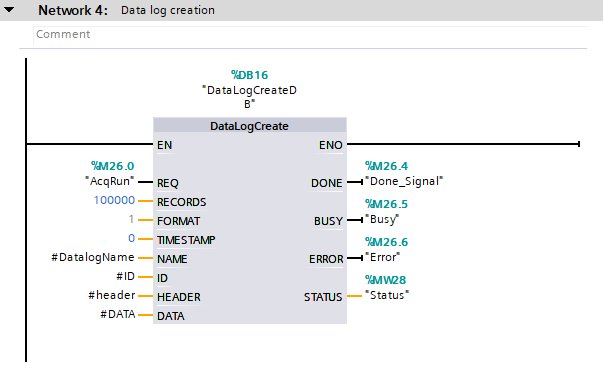
\includegraphics[width=0.5\textwidth,clip,trim={0 0 3cm 0}]{tutorial/create}
%   \caption{DataLogCreate block.}
%   \label{fig:datalogcreate}
% \end{figure}

% \begin{figure}[H] \centering
%  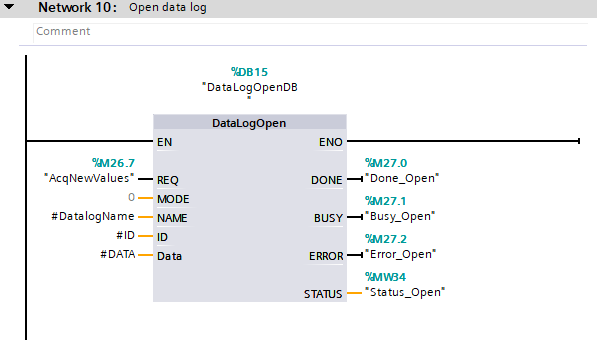
\includegraphics[width=0.5\textwidth,clip,trim={0 0 3cm 0}]{tutorial/open}
% \caption{DataLogOpen block.}
%   \label{fig:datalogopen}
% \end{figure}

% \begin{figure}[H] \centering
% 	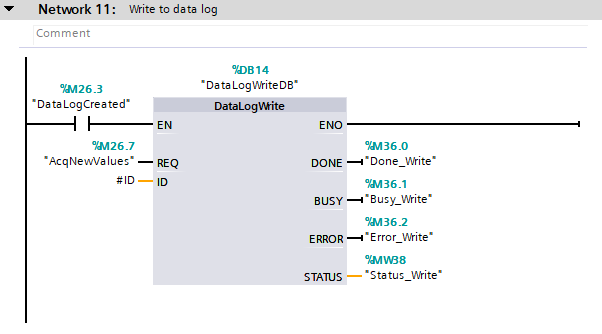
\includegraphics[width=0.5\textwidth,clip,trim={0 0 3cm 0}]{tutorial/write}
% 	\caption{DataLogWrite block.}
% 	\label{fig:datalogwrite}
% \end{figure}

% \begin{figure}[H] \centering
%  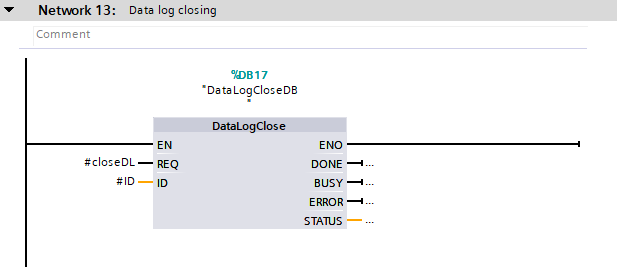
\includegraphics[width=0.5\textwidth,clip,trim={0 0 3cm 0}]{tutorial/close}
%   \caption{DataLogClose block.}
%   \label{fig:datalogclose}
% \end{figure}

% \begin{figure}[H] \centering
%  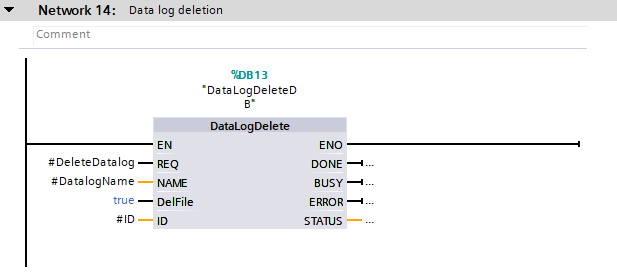
\includegraphics[width=0.7\textwidth,clip,trim={0 0 3cm 0}]{tutorial/delete}
%   \caption{DataLogDelete block.}
%   \label{fig:datalogdelete}
% \end{figure}

\begin{figure}[H] \centering
\begin{minipage}{.45\textwidth}
  \centering
 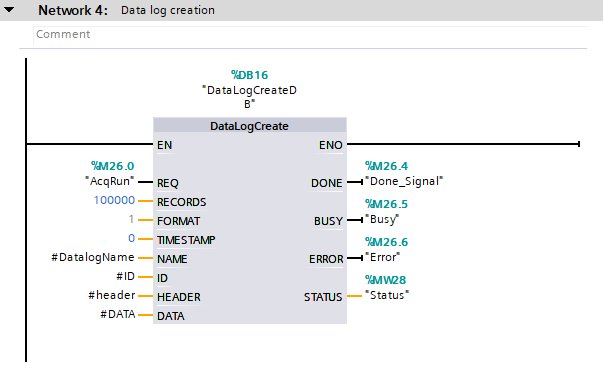
\includegraphics[width=\textwidth,clip,trim={0 0.8cm 3cm 0}]{tutorial/create}
  \caption{DataLogCreate block.}
  \label{fig:datalogcreate}
\end{minipage}
% 
\begin{minipage}{.45\textwidth}
  \centering
 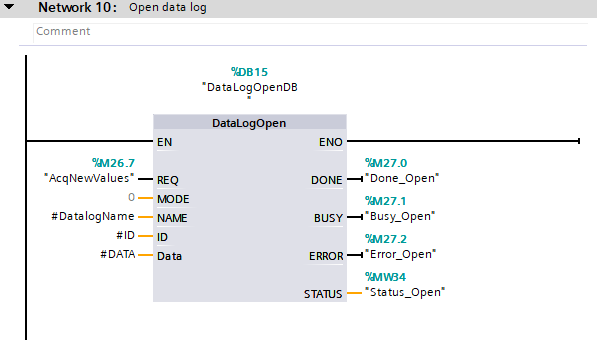
\includegraphics[width=\textwidth,clip,trim={0 0.4cm 3cm 0}]{tutorial/open}
\caption{DataLogOpen block.}
  \label{fig:datalogopen}
\end{minipage}
\end{figure}

\begin{figure}[H] \centering
\begin{minipage}{.45\textwidth}
  \centering
	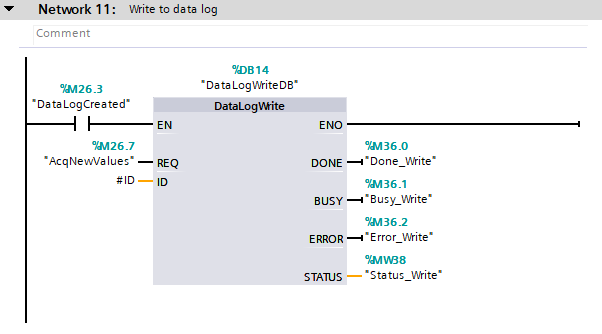
\includegraphics[width=\textwidth,clip,trim={0 0 3cm 0}]{tutorial/write}
	\caption{DataLogWrite block.}
	\label{fig:datalogwrite}
\end{minipage}
% 
\begin{minipage}{.45\textwidth}
  \centering
 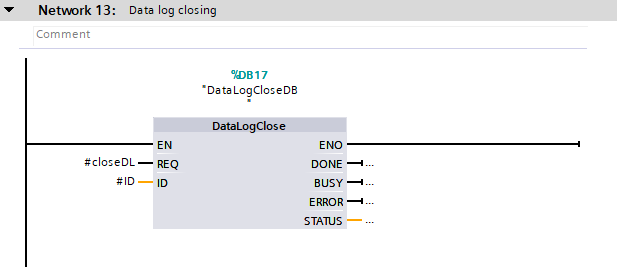
\includegraphics[width=\textwidth,clip,trim={0 -2cm 3cm 0}]{tutorial/close}
  \caption{DataLogClose block.}
  \label{fig:datalogclose}
\end{minipage}
\end{figure}


\begin{figure}[H] \centering
\begin{minipage}{.45\textwidth}
  \centering
 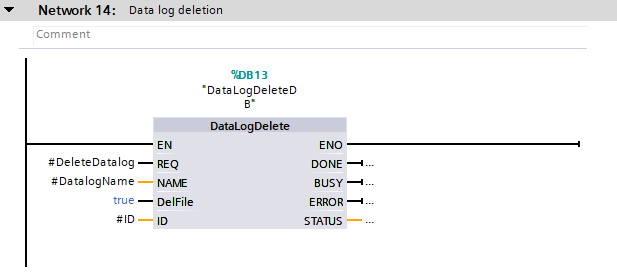
\includegraphics[width=\textwidth,clip,trim={0 0 3cm 0}]{tutorial/delete}
  \caption{DataLogDelete block.}
  \label{fig:datalogdelete}
\end{minipage}
\end{figure}
The actions performed by these blocks are: Create the \verb|.csv| file, open the
file to be written, write data to the file, close the file, and delete the file. 
The inputs and outputs of these blocks are used to determine the information
about the \verb|.csv| file and the data to be stored.
% Most of the inputs and outputs of the presented blocks are similar.
So, the function
of these inputs and
outputs will be presented in the following paragraphs.

The \verb|REQ| input triggers the action to be performed using the rising edge
of its corresponding variable.
In order to identify the file to be manipulated, the \verb|ID| and \verb|NAME|
inputs are used. These inputs use a unique id number and a string, respectively. This string is used as the name of the
\verb|.csv| stored in the SD card.

The \verb|DATA| input receives the data to be stored in the \verb|.csv| file.
The data is structured in a variable of type struct. The struct type can contain variables of different type and size, for instance: a struct can contain a boolean,
an int, a word
and a string.

The \verb|HEADER| input is a string to be \emph{prepended} to the first line of
the \verb|.csv| file. The first line of the file identifies the
stored variables. As this string variable will be part of the \verb|.csv| file, it is needed to
include commas ``,'' inside it to separate the identifiers of the variables.

\begin{observation}
  \label{obs:stringSize}
 As the string type has variable size, it is important to take into account its
 maximum size, that is $256$ Bytes. That means that it can store up to 256 characters,
 considering the commas.
\end{observation}

The \verb|TIMESTAMP| input is used to identify if a timestamp column will be inserted or not in the \verb|.csv|. A boolean variable is
used to set the column. If the variable is \emph{true} the column is added, otherwise it
is not.

The outputs \verb|DONE|, \verb|BUSY|, \verb|ERROR| and \verb|STATUS| are not used
in this work, but they can be used to identify the status of the action to be
performed. The status of each data log function block can be the following: the action is being
performed (BUSY), the action is done (DONE) or an error occurred (ERROR). Each
status has its corresponding boolean output. If an error occurred, \verb|STATUS| outputs
a code to identify the error. This code is used for troubleshooting
and can be found in the Siemens manual, \cite{datalogSiemens}.

In order to organise the data used for all these blocks, a \emph{DataBlock} was
used. The structure of this \emph{DataBlock} is shown in \Autoref{fig:exampleDataBlock}. We can see in this \emph{DataBlock} the main variables used to create
and write the log data: \verb|DATA|, \verb|HEADER|, \verb|ID| and \verb|NAME|.


\begin{figure}[H] \centering
 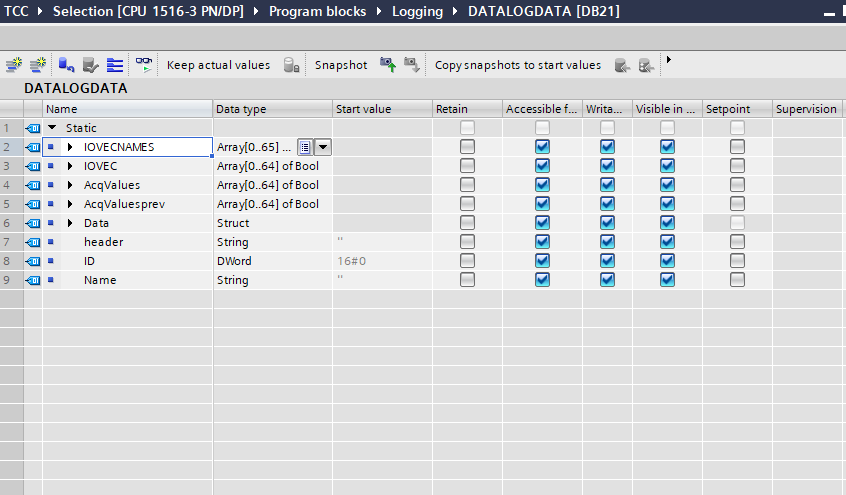
\includegraphics[width=\textwidth]{tutorial/datalog.png}
  \caption{Example of DataBlock used to log data.}
  \label{fig:exampleDataBlock}
\end{figure}


In this work, we need to store the input\slash output
vectors of the controller. The \emph{IOvectors} (input\slash output vectors) are composed by
boolean variables. One restriction to the storage of these vectors is that there
must not be two consecutive vectors with the same data.

In order to achieve the needs of the project, a
function block was created to be used in the \LD. This new function block uses
the data log function blocks from \Crefrange{fig:datalogcreate}{fig:datalogdelete} and some additional logic. This function block is called \emph{LOGDATA}, and it is
depicted in
\Autoref{fig:logdataBlock}.
\begin{figure}[H] \centering
 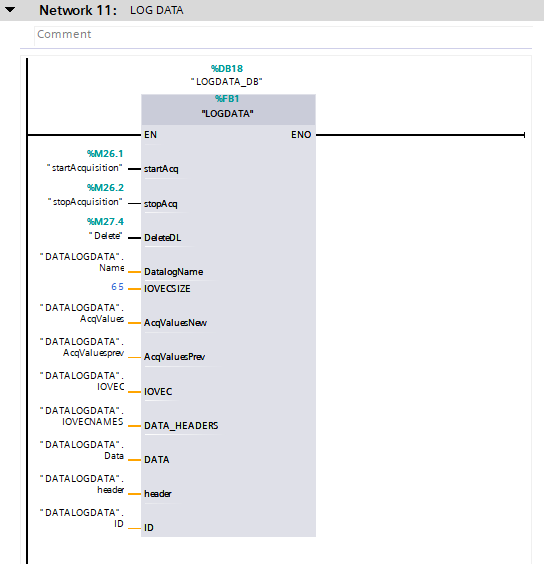
\includegraphics[width=0.7\textwidth]{tutorial/logdata.png}
  \caption{LOGDATA block.}
  \label{fig:logdataBlock}
\end{figure}
The 12 inputs of the \emph{LOGDATA} block will be briefly described in the following paragraphs. And after that, the logic used to implement the block will be presented.

The \verb|startAcq|,
\verb|stopAcq| and \verb|DeleteDL| inputs are used to start and stop the
acquisition and to
delete the \verb|.csv| file, respectively. The \verb|DatalogName| input represents the name of the file. \verb|IOVECSIZE| identifies the number of variables to
be stored.
In order to avoid two equal consecutive \emph{IOvectors}, two arrays are
created : \verb|AcqValuesNew| and
\verb|AcqValuesPrev|. These two variables store the current \emph{IOvector} and the preceding one, respectively. These arrays are compared to each other, and if
they differ, \verb|AcqValuesNew| is stored in the \verb|.csv| file. 
 The value of these arrays is
changed from inside the block via an update block.

\verb|IOVEC| is also an input that is changed from inside the block. It
is used as a buffer for the vectors. The data of this buffer is periodically copied to the variable connected to the
\verb|DATA| input. \verb|DATA|, in turn, is internally connected to the
\verb|DATA| input of the data log function blocks. 

Instead of writing the tags of the variables in the \verb|HEADER| input string, a \verb|DATA_HEADERS| input is created.
An array of strings of size \verb|IOVECSIZE| is created and connected to \verb|DATA_HEADERS|. This array contains the tags of all variables to be
stored in \verb|DATA|. The contents of the array are concatenated with
commas placed between them, and a new string is created. This new string is assigned to the variable
\emph{header}, connected to the \verb|HEADER| of the data log function blocks. 

An example of the data stored in this work can be seen in
\Autoref{fig:exampleDataStruct}. In this figure is possible to notice that the data structure is composed of variables whose tags are shown
in \Autoref{sec:implementation}. 
\begin{figure}[H] \centering
 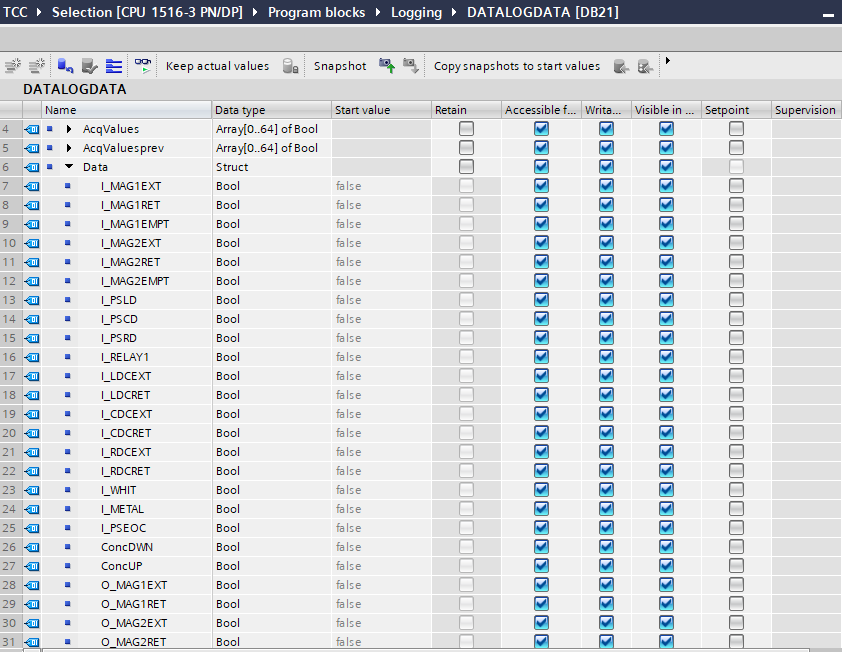
\includegraphics[width=\textwidth]{tutorial/datalogdata2.png}
  \caption{Example of Data struct.}
  \label{fig:exampleDataStruct}
\end{figure}
The code inside the \verb|LOGDATA| block uses the following logic.
First the value of \verb|AcqValuesNew| is copied to \verb|AcqValuesPrev|. Then \verb|AcqValuesNew| is updated with the values of the inputs\slash outputs of the controller. After that, \verb|AcqValuesNew| and \verb|AcqValuesPrev| are compared and if they differ, \verb|AcqValuesNew| is prepared to be stored.
Once the data is prepared, it is stored in the file. 
The last step, storage in the file, is made using the data log function blocks depicted in
\Crefrange{fig:datalogcreate}{fig:datalogdelete}. The other steps will be shown
in the next paragraphs.

The copy of the values from the \verb|AcqValuesNew| array is made by using the \mbox{\emph{MOVE\_BLK}} function block present in the Siemens \PLC. 
In order to update the values of \verb|AcqValuesNew|, the custom function block called
\emph{UpdateValues} is created inside \emph{LOGDATA}. This block can be seen in
\Autoref{fig:updateValuesBlock}. The code of this block is programmed using the \SCL{} language. In \Autoref{fig:updateValuesBlockCode} we
can see the code of the \mbox{\emph{UpdateValues}} function block.

\begin{figure}[H] \centering
 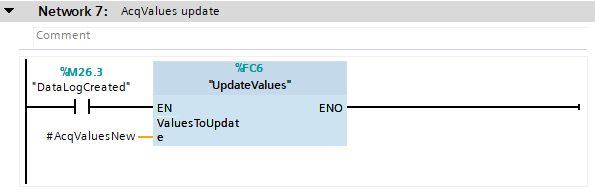
\includegraphics[width=0.7\textwidth]{tutorial/updateValues.png}
  \caption{UpdateValues block.}
  \label{fig:updateValuesBlock}
\end{figure}

\begin{figure}[H] \centering
 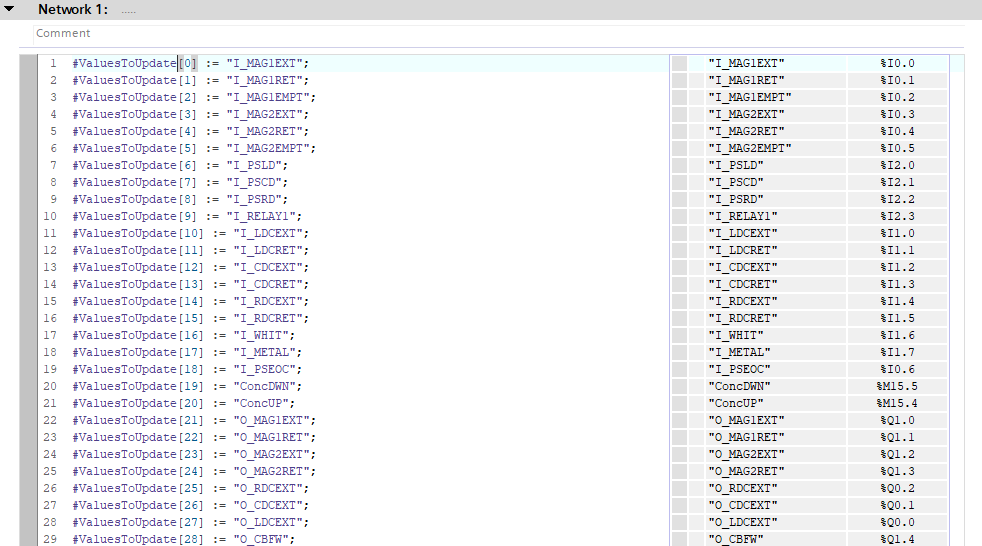
\includegraphics[width=\textwidth]{tutorial/updateValues2.png}
  \caption{Code inside UpdateValues block.}
  \label{fig:updateValuesBlockCode}
\end{figure}

In order to compare \verb|AcqValuesNew| and \verb|AcqValuesPrev|, a
\emph{CompareArrays} block is created, in which all the values of both arrays are compared
bitwise. And if they are different, the
\verb|AcqValuesNew| is copied to the temporary variable input to \verb|IOVEC|, the buffer.
This logic can be seen in \Autoref{fig:compareArrayBlock}.

\begin{figure}[H] \centering
 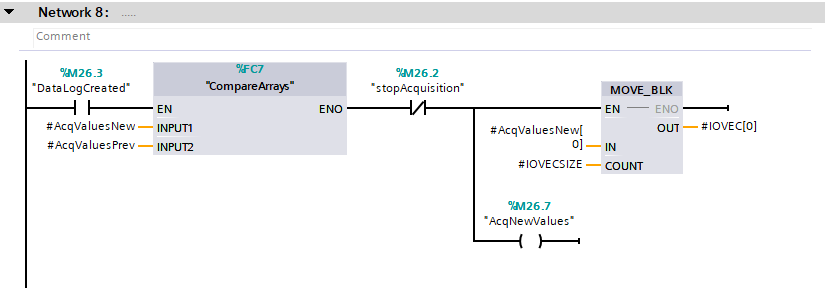
\includegraphics[width=\textwidth]{tutorial/compareArray}
  \caption{CompareArrays block.}
  \label{fig:compareArrayBlock}
\end{figure}

Before using the blocks depicted in \Crefrange{fig:datalogcreate}{fig:datalogdelete} to create the \verb|.csv| file and store the data, the data in the temporary
variable \verb|IOVEC| is copied to \verb|DATA|. The copy is carried out by using the custom function block
\emph{PutInDataStruct} shown in \Autoref{fig:putInDataStructBlock}. The code of this block is also programmed using \SCL{} and it is represented in \Autoref{fig:putInDataStructBlockCode}.  

\begin{figure}[H] \centering
 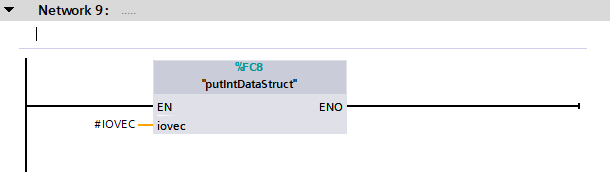
\includegraphics[width=0.7\textwidth]{tutorial/putindatastruct.png}
  \caption{PutInDataStruct block.}
  \label{fig:putInDataStructBlock}
\end{figure}

\begin{figure}[H] \centering
 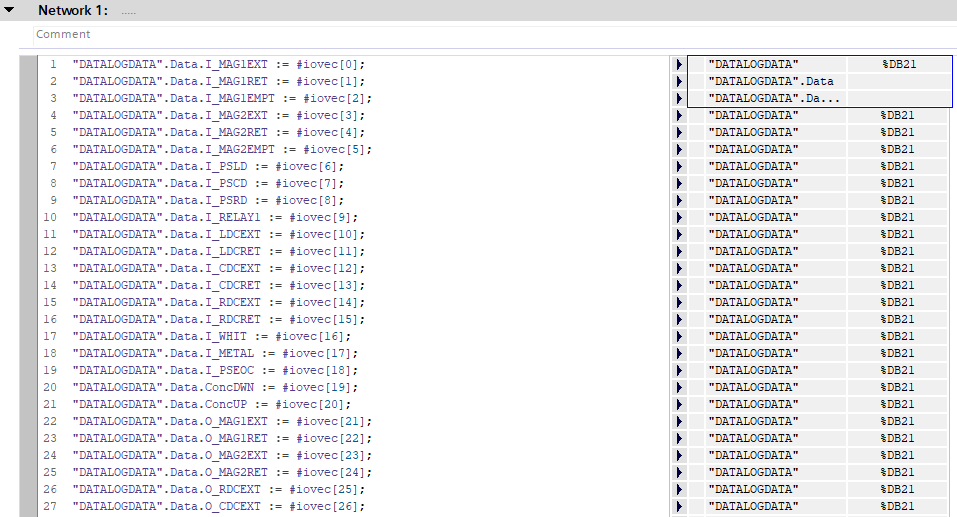
\includegraphics[width=\textwidth]{tutorial/putindatastruct2.png}
  \caption{Code inside PutInDataStruct block.}
  \label{fig:putInDataStructBlockCode}
\end{figure}

\begin{observation}
  Since the tags are divided between the 2 \PLCs{}, in order to have all tags in
  a same \PLC, ``Get'' and ``Put'' blocks were used. Two Data blocks
  are used to store the inputs and outputs of the Handling-Assembly-Storage \PLC{} and send\slash receive data using those function blocks.
  % One datablock is used to send the data to other PLC and another to receive.
 Each data block is located in a different \PLC.
 The aspect of these data blocks can be seen in \Autoref{fig:iovecFromPlc,fig:iovecFromPlctwo}
\end{observation}
\begin{figure}[H] \centering
\begin{subfigure}[h]{\textwidth} \centering
 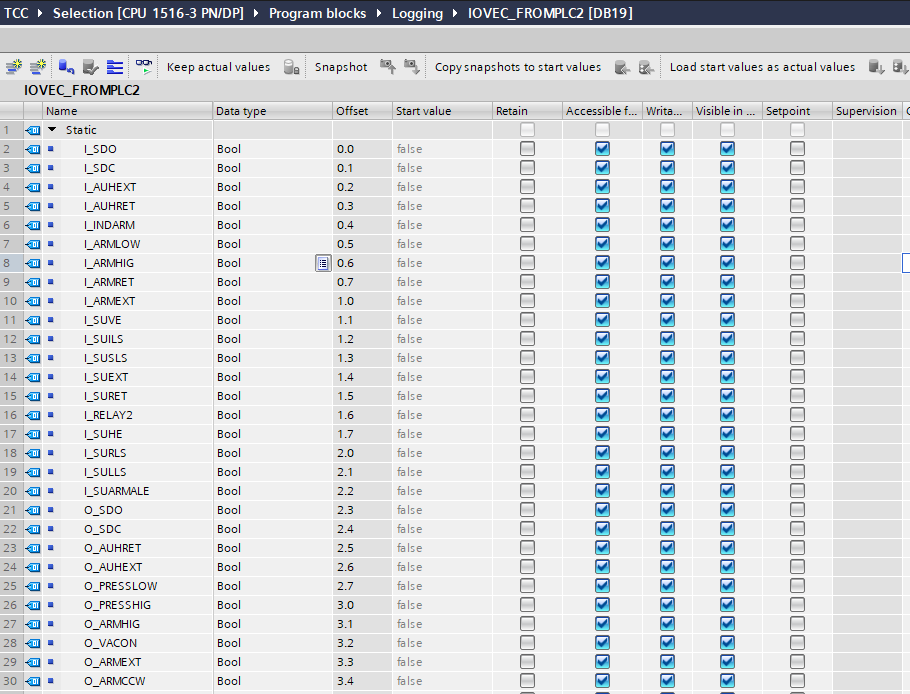
\includegraphics[width=\textwidth]{tutorial/iovecfromplc2.PNG}
  \caption{IOVEC\_FROMPLC2 DataBlock.}
  \label{fig:iovecFromPlc}
\end{subfigure}
\begin{subfigure}[h]{\textwidth} \centering
 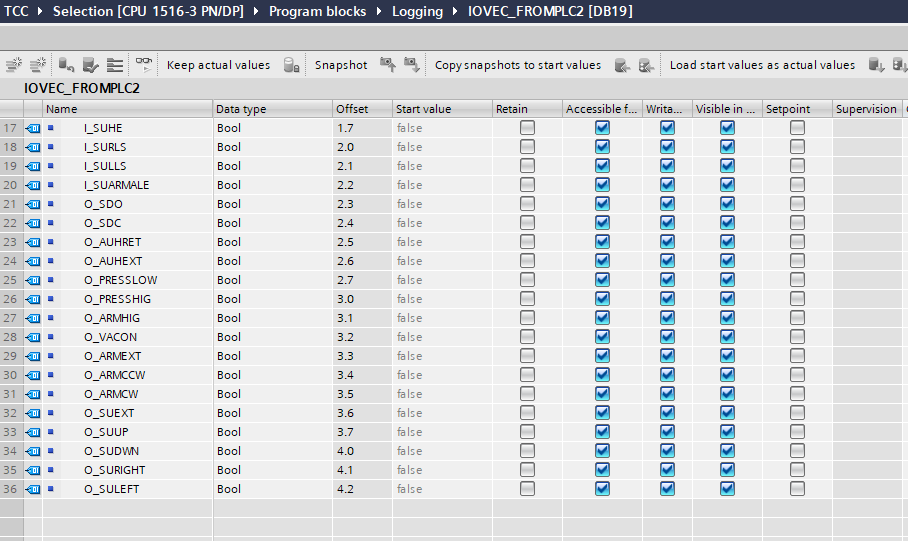
\includegraphics[width=\textwidth,clip,trim={0 1cm 0 0}]{tutorial/iovecfromplc2-1.PNG}
  \caption{IOVEC\_FROMPLC2 DataBlock - Continuing.}
  \label{fig:iovecFromPlctwo}
\end{subfigure}
\caption{Inputs\slash Outputs from Handling-Assembly-Storage \PLC.}
\end{figure}
% \subsection{HMI}
% \cite{webserverSiemens,userdefinedwebpagesSiemens}
% As a tool to facilitate the control of the system and the start and stop of acquisition, it was created a web page that is used as an  \HMI. It was created
% based on a bootstrap example\footnote{the example is available
%   at\url{https://getbootstrap.com/docs/4.3/examples/floating-labels/}}, and the
% html tags shown in the tutorial present in \cite{userdefinedwebpagesSiemens} using the a standard web page with the bootstrap buttons 

% \begin{figure}[H] \centering
%  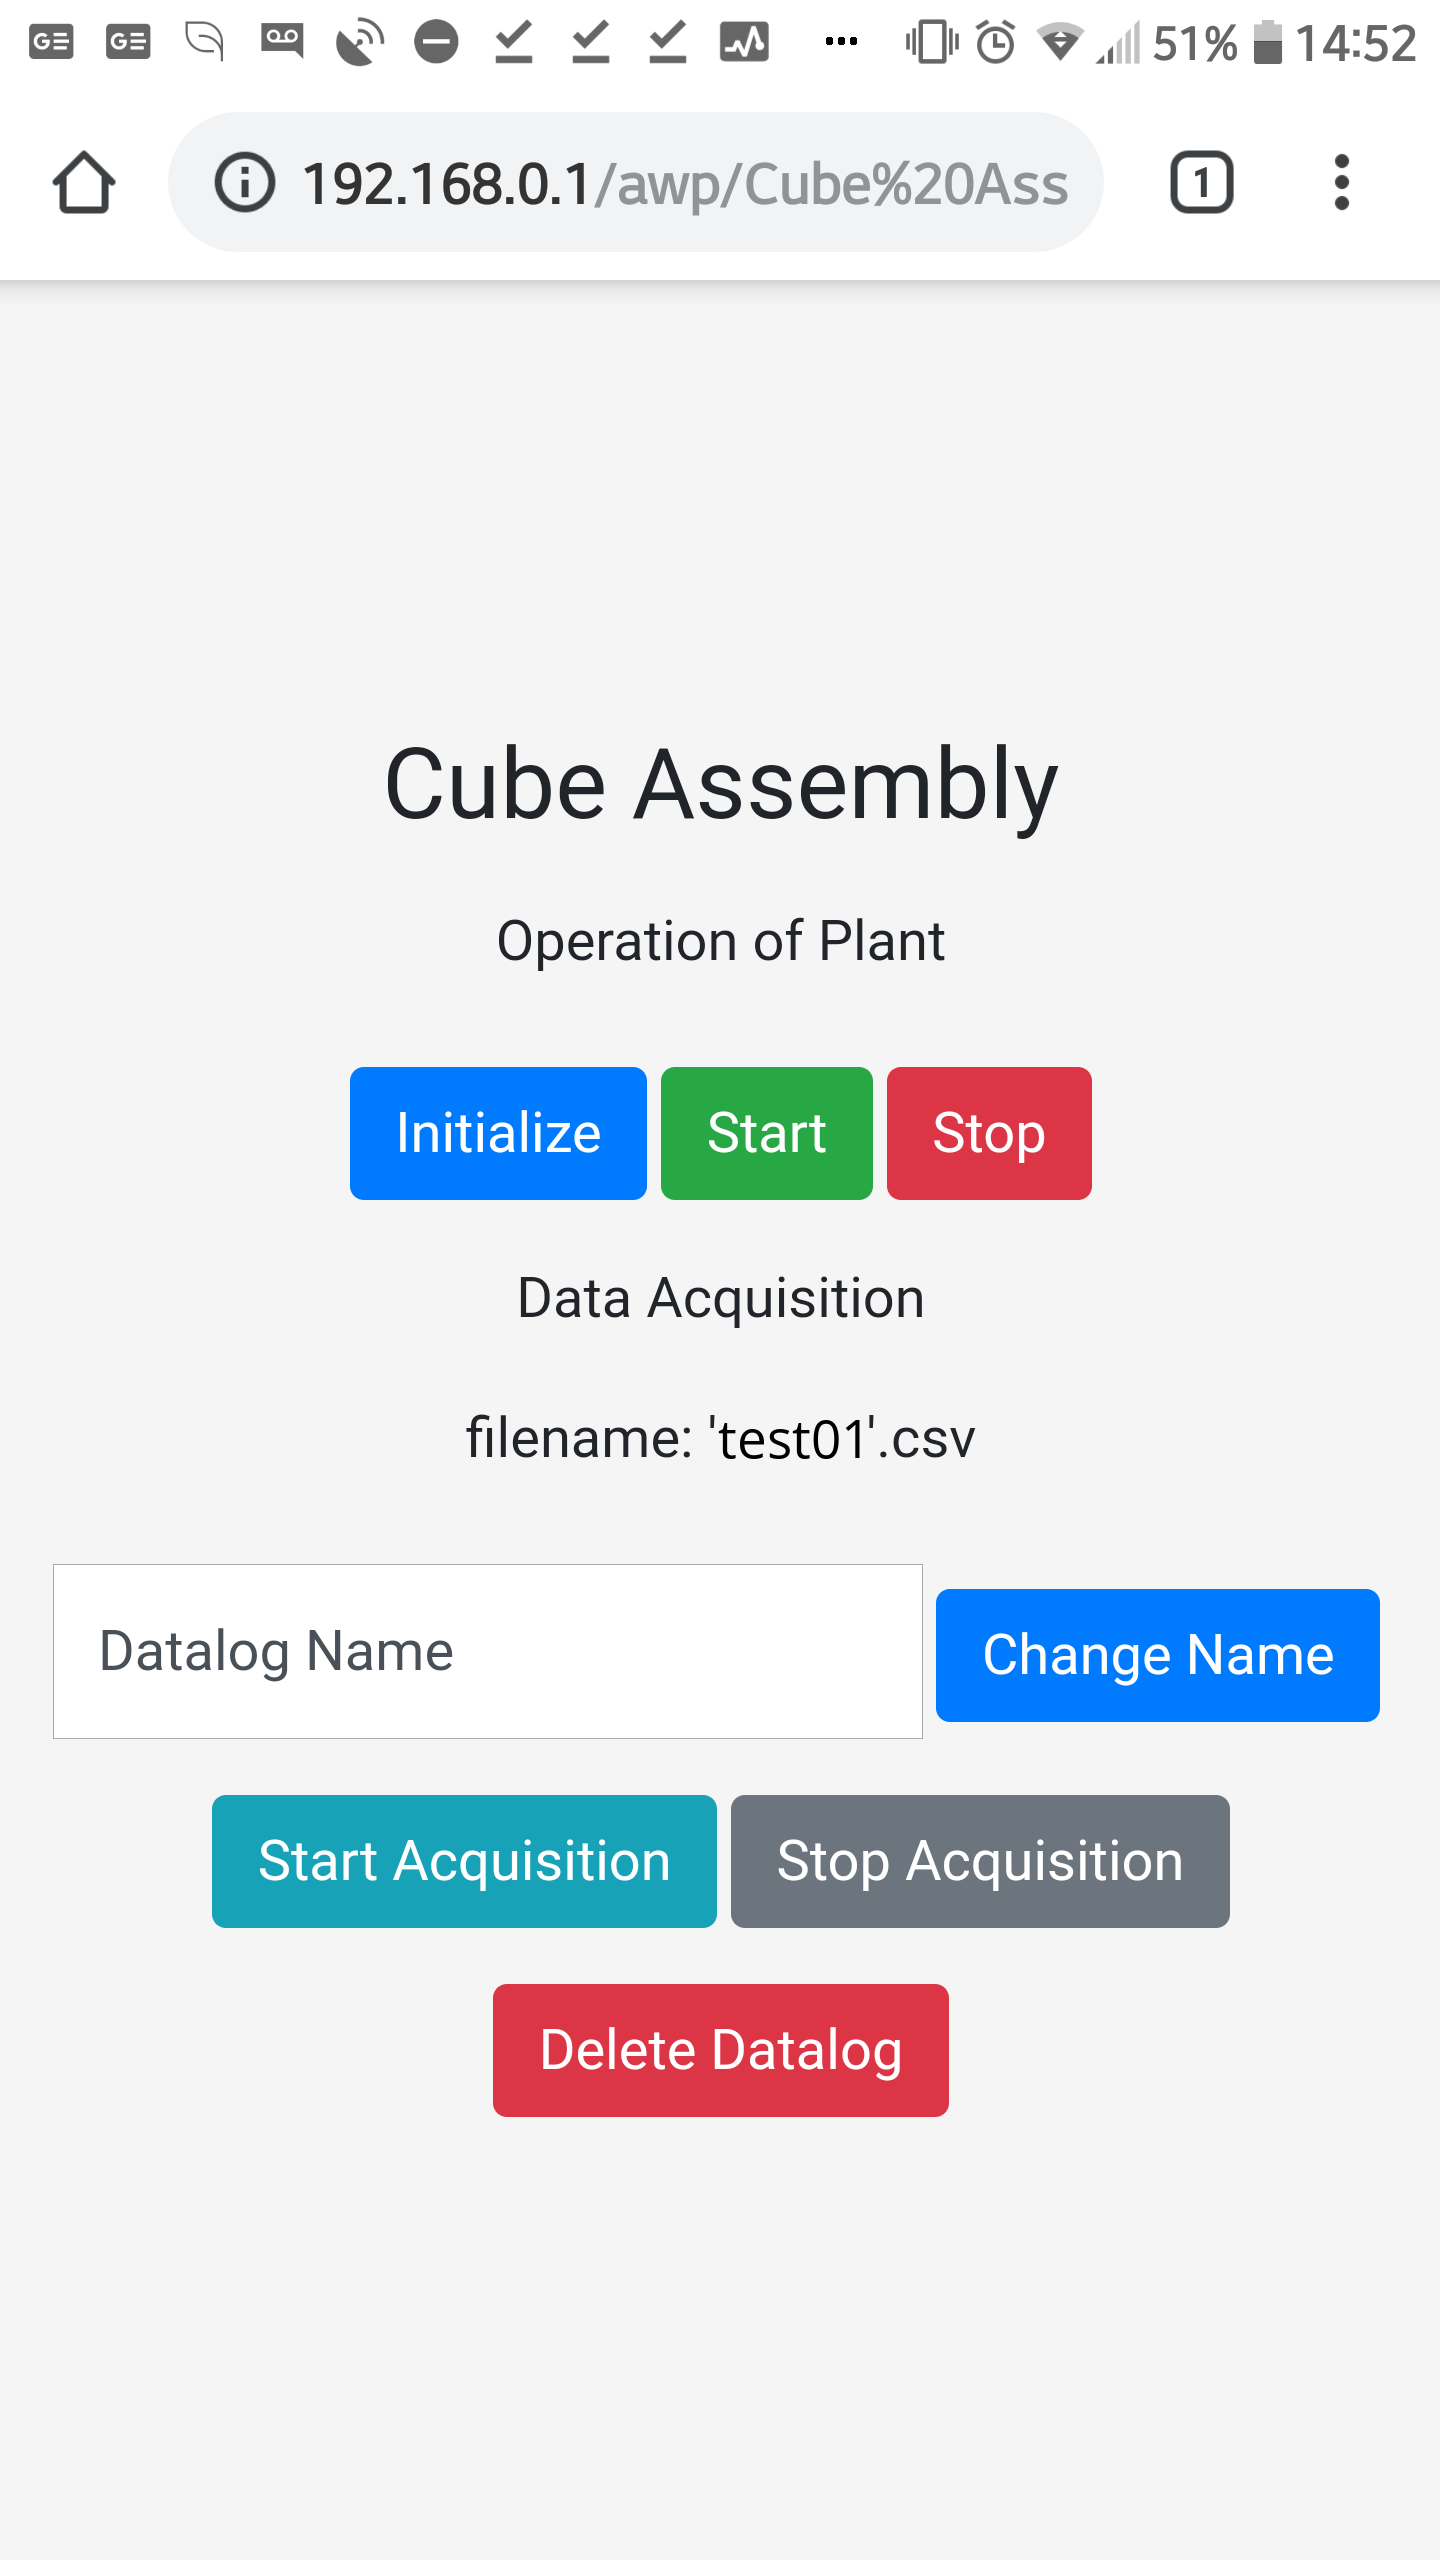
\includegraphics[height=0.6\textwidth]{hmi_mobile2}
%   \caption{HMI on mobile.}
%   \label{fig:hmi_mobile}
% \end{figure}
% \begin{observation}
%   Since this is the first version of the block, that are still lots of
%   improvements to be made to optimise its use. Some variables can be changed, in
%   order to be used as 
%   internal variables, instead of creating new variables in a DataBlock. And
%   maybe some variables and even rungs can be removed or substituted.
% \end{observation}
\section{Model Identification}
\label{sec:modIdent}
 Once the data is logged, the \verb|.csv| file can be downloaded from a Web Server or from the SD card. Following the steps shown in the Siemens Manual,
\cite{webserverSiemens}, it is possible to configure a web server in the Siemens
\PLC{} S7-1500. And once the web server is configured, the file can be downloaded in different
ways, most of them are shown in section 3.13 of the same manual, \cite{webserverSiemens}. In this work, the \verb|.csv| file was downloaded from the terminal of a computer connected to the same network of the \PLC{}.
The commands that can be used to download the file from the terminal are the following:
\vspace{-1cm}
\begin{lstlisting}[language=bash,numbers=none]
  $ wget --content-disposition -i "http://192.168.2.132/DataLogs?Action=LIST"
\end{lstlisting}
and
\vspace{-1cm}
\begin{lstlisting}[language=bash,numbers=none]
  $ curl -k "https:///192.168.2.132/Filebrowser?Path=/DataLogs/name_of_the_file.csv&RAW" -H "Referer: https://192.168.2.132/Portal/Portal.mwsl?PriNav=Filebrowser&Path=/DataLogs/"
\end{lstlisting}
Where the address ``192.168.2.132'' should be the address of the \PLC{} in which
the web server is running and ``name\_of\_the\_file.csv'' should be the name of the file.

Once the \verb|.csv| is downloaded to the PC, the paths can be obtained from the data and the identification algorithm can
be executed. The acquisition of the paths and the identification algorithm, \Autoref{alg:identification}, were
implemented in python.

Since the identification is
performed by using a black box approach, we do not have any previous information of what is
considered a path in the file. So, the first vector is considered as the initial
vector, and every time it is repeated in the file another path is created.
Once the paths are obtained they are modified using \Autoref{eq:modifiedPath,eq:modifiedPathb}.

A brief example of this method of path acquisition can be presented. Consider the observed data of the example shown in \Autoref{sec:identification}, is in the following
\verb|.csv| file:

\lstinputlisting[caption=CSV file generated from example of \Autoref{sec:identification}.]{../../figures/example/example.csv}

Using the method proposed, the vector $\colvec{1&0&0}^ T$ is considered as the initial vector and 4 paths are obtained from the file:
\setlength\arraycolsep{2pt}
\begin{align*}
  p_1&= \left(\colvec{1\\0\\0},a,\colvec{1\\1\\0},b,\colvec{0\\1\\1},c,\colvec{0\\0\\0},d,\colvec{0\\0\\1},e,\colvec{1\\0\\0}\right) \\
  p_2&= \left(\colvec{1\\0\\0},g,\colvec{0\\0\\0},h,\colvec{1\\1\\0},b,\colvec{0\\1\\1},c,\colvec{0\\0\\0},i,\colvec{1\\0\\0}\right) \\
  p_3&= \left(\colvec{1\\0\\0},j,\colvec{0\\1\\1},l,\colvec{1\\0\\0}\right) \\
  p_4&= \left(\colvec{1\\0\\0},g,\colvec{0\\0\\0},h,\colvec{1\\1\\0},b,\colvec{0\\1\\1},i,\colvec{1\\1\\1},m,\colvec{0\\0\\0},d,\colvec{0\\0\\1},n,\colvec{1\\1\\0}\right) \\
\end{align*}
If we compare these paths with those shown in \Autoref{sec:identification},
we can see that using this method, 4 paths are obtained instead of the 3 paths presented in \Autoref{sec:identification}.
If we analyse the path $p_2$ from \Autoref{sec:identification}, we can notice that the vector $\colvec{1&0&0}^ T$ is repeated inside the path :
\begin{align*}
  p_2&= \left(\colvec{1\\0\\0},g,\colvec{0\\0\\0},h,\colvec{1\\1\\0},b,\colvec{0\\1\\1},c,\colvec{0\\0\\0},i,{\color{gray} \colvec{1\\0\\0}},j,\colvec{0\\1\\1},l,\colvec{1\\0\\0}\right) \\
\end{align*}
Since is not possible to have a repeated vector in a path using the method proposed, this path $p_2$ is divided in two, resulting on the $p_2$ and $p_3$ of this section. 

 The change in the number of paths is reflected on the
 identified model. Choosing $k=1$ and $k=2$ for the modified paths and executing the identification algorithm, the models depicted in \Autoref{fig:identExamplekone,fig:identExamplektwo} were obtained.
Comparing the state transition diagram of these models with those shown in \Autoref{fig:examplek1,fig:examplek2}, we can see the difference
caused by the additional path in the identified model.
\begin{figure}[H]
  \centering
  \includegraphics[width=\textwidth]{example/examplek1NoArrows}
  % \includetikzfigure[width=\textwidth]{example/stdin}
  \caption{Identified model from paths extracted from \texttt{.csv} file using $k=1$.}
  \label{fig:identExamplekone}
\end{figure}

\begin{figure}[H]
  \centering
  \centering
  \includegraphics[width=\textwidth]{example/examplek2NoArrows}
  % \includetikzfigure[width=\textwidth]{example/examplek2}
  \caption{Identified model from paths extracted from \texttt{.csv} file using $k=2$.}
  \label{fig:identExamplektwo}
\end{figure}

The path acquisition method presented in this work is used in the identification of the manufacturing system and its results are discussed in the next chapter. 
The tools created to implement the path acquisition method and the
identification algorithm are presented in Appendix \ref{sec:daoct}.


%%% Local Variables:
%%% mode: latex
%%% TeX-master: "../monografia"
%%% End: